%%%%%%%%%%%%%%%%%%%%%%%%%%%%%%%%%%%%%%%%%%%%%%%%%%%%%%%%%%%%%%%%%%%%%%%%%%%%%%%%
\chapter{Introduction}\label{ch:introduction}
%%%%%%%%%%%%%%%%%%%%%%%%%%%%%%%%%%%%%%%%%%%%%%%%%%%%%%%%%%%%%%%%%%%%%%%%%%%%%%%%

%3nd-review
\section{State of Affairs and Motivation}\label{sec:state-of-the-art}
 

Emerging technologies such as SDN and NFV are great promises. If succeeding at large-scale, they would change drastically the development and operation of computer networks. But, especially on NFV, its enabling technologies such as virtualization still pose challenges on performance,  reliability, and security\cite{nfv-challenges}. Closed hardware solutions are easier to pass on Service Layer Agreement since they have a much more predictable behavior. Since it is expected virtualization to impact negatively on performance, these VNFs have to keep its degradation as small as possible. Guarantee the Service Layer Agreements on emerging scenarios is now a harder question. There is a demand for more reliable methods to ensure the SLAs, over different types of loads.


It is already a well-known fact that the type of traffic used on performing tests matters. Studies show that a realistic Ethernet traffic provides a different and more variable load characteristics on routers\cite{harpoon-validation}, even with the same mean bandwidth consumption. It indicates that tests with constant bit rate traffic generator tools are not enough for a complete validation of new technologies. There are many reasons for this behavior, which includes burstiness and packet sizes.


A burstier traffic can cause packet more buffer overflows on network \cite{burstiness-queue-lenght} \cite{modelling-of-self-similar} \cite{empirical-interarrival-study}, degenerating network performance\footnote{Fuatures such as packet-trains periods and inter-packet times affect traffic burstiness}, and  measurement accuracy\cite{legotg-paper} \cite{background-traffic-matter}. Another key question is how applications will deal with packets. It is a well-known fact that applications have a huge performance degradation processing small packets\cite{comparative-trafficgen-tools}. A realistic synthetic traffic must not have a single packet-size but must use a distribution \cite{packet-distribution-model}. 


Realistic workload generators are also essential security research\cite{ditg-paper}.  Generation of realistic workloads is important in the evaluation of firewall middleboxes. It includes studies of intrusion, anomaly detection, and malicious workloads\cite{ditg-paper}. 

Since on traditional hardware-based types of \textit{middleboxes}, the impact of realistic traffic is not negligible; we can expect that its impact over virtualized middle-boxes should be even larger, due the extra overhead of a virtualization layer. 


Another critical point is the flow-oriented operation of SDN networks. Each new flow arriving on an SDN switch demands an extra communication load between it and the controller. This may create a bottleneck between the switch and the controller.  Also the SDN switches have a flow-oriented operation. Since its operation relies on queries on flow tables, a stress load must have the same flow properties of an actual Internet Service Provider.


Therefore, there is a demand for the study of the impact of a realistic traffic on this new sort of environment. How VNFs and virtualized middle-boxes and SDN testbeds will behave if stressed with a realistic traffic load in comparison to a constant rate traffic is a relevant subject. 


\section{Open-source Solutions}


The open-source community offers a huge variety of workload generators and benchmarking tools \cite{ditg-paper}\cite{validate-trafficgen}\cite{comparative-trafficgen-tools}\cite{performance-trafficgen}. Most of these tools were built for specific purposes and goals, so each uses different methods of traffic generation, and enable controll of different features, such as throughput (bits/bytes per second, packets per seconds), packet-sizes, protocols and header customization, payload customization, inter-packet times, On/Off periodos, start and sending time, and emulation of applications such as Web server/client communication, VoIP, HTTP, FTP, p2p applications, and many more.


Some traffic generator tools offer support emulation of single application workloads. But this does not correspond to real complex scenarios. Other tools work as packet replay engines, such as TCPreplay and TCPivo. Although in that way is possible to produce a realistic workload at high rates, it comes with some issues. First, the storage space required becomes huge for long-term and high-speed traffic capture traces. Also, obtaining good traffic traces sometimes is hard, due privacy issues and fewer good sources. Many tools support a larger set of protocols and high-performance, such Seagull and Ostinato. Others are also able to control inter-packet times and packet sizes using stochastic models, like D-ITG\cite{ditg-paper} and MoonGen. 


We have available have a variety of APIs that enable creation of traffic and custom packets, wich include low-level APIs, such as Linux Socket API,  Libpcap, Libtins, DPDK, Pcapplusplus, libcrafter, impacket, scapy and many others. These APIs enable a finer controll and customization over each packet, and are used to implement traffic generators. For example, Ostinato and TCPreplay uses Libpcap, and MoonGen uses DPDK. Also, many traffic generators provides their own API, such as Ostinato Python API, D-ITG C API, and MoonGen LUA API. 


%They can give a good control of the traffic and high rates. Es example of controllable features we can list:
%\begin{itemize}
%\item Throughput, the number of bytes, number of packets.
%\item Protocols. Most of the tools give support to network and transport protocols. Many also offer support to Link and Application protocols;
%\item Header and payload configuration. Support for header customization includes source and destination port/addresses, QoS parameters, flags, etc. Some traffic generators also allow customizing payload bytes.
%\item Inter-packet times. Some tools offer a set of stochastic distributions to control inter-packet times. The user can use these stochastic functions to emulate realistic inter-arrival times.
%\item On/off periods: support of packet trains periods. Many offer stochastic models to control it. 
%\item Sending time and start-time: the user can use these features to control flows timings.  
%\item Packet-size: support for different packet sizes. Some tools offer constant values or stochastic distributions to control packet sizes.
%\item Paralell flows configuration.
%\item Emulation of specific applications: common examples are 
%\end{itemize}


If the user whats to reproduce an realistic traffic scenatio, since there is so many features and tools, selecting a good configuration is by itself a complex research project. How to use each parameter to simulate a specific scenario is a hard question \cite{legotg-paper}\cite{selfsimilar-ethernet}. It is a manual process and demands implementation of scripts or programs leveraging human (and scarce) expertise on network traffic patterns and experimental evaluation. Also, having a good compromisse between quality of realism, progamming time and scalability another challange. Since this is a complex process, a simplistic and less time-expensive sollution is choosen over a a realistic and acuratter but comple and time-costly sollution. 


Some sollutions exists on the open-source comunity. Some tools like Swing and Harpoon uses capture traces to set intern parameters, enabling an easier configuration. Also, Swing uses complex multi-levels models which are able to provide a high degree of realism\cite{swing-paper}. But they have their issues as well. Harpoon does not configure parameters at packet level\cite{harpoon-paper} and is not supported by newer Linux kernels, what may be a huge problem with setup and configuration. Swing\cite{swing-paper} aims to generate realistic traffic, but focous on background traffic, and high throughputs it is not a goal off the application\cite{swing-paper} \cite{legotg-paper}. Due the fact that its traffic generation engine is coupled to its modeling framework, you can't opt to use a newer/faster packet generation library. The only way of replacing the traffic engine is changing and recompiling the original code. And this is a hard task\cite{legotg-paper}.


%Since synthetic traffic traces generation is mature in academia, the creation of custom network workloads through the configuration of  open-source tools is an affordable task. But it is not often available in an automatic way, and most of the times is a challenging question\cite{legotg-paper}, and still, requires expert knowledge. It requires time, study, and is vulnerable to human mistakes and lack of validation. Such work may require weeks to complete a realistic reproduction of a single scenario, so most of the time it is just not done. We argue that widely (i.e. affordable) existing approaches can be regarded as simplistic often point solutions to more general cases. 


% Also, just choosing which workload generator tool may fit better for the user needs is not a simple question. Tools like D-ITG\footnote{\href{http://traffic.comics.unina.it/software/ITG/}{http://traffic.comics.unina.it/software/ITG/}} provide support to many different stochastic functions, Ostinato\footnote{\href{http://ostinato.org/}{http://ostinato.org/}} provides a larger support for protocols, and a higher throughput for each thread\cite{comparative-trafficgen-tools}, and others like Seagull\footnote{\href{http://gull.sourceforge.net/doc/WP_Seagull_Open_Source_tool_for_IMS_testing.pdf}{http://gull.sourceforge.net/doc/WP\_Seagull\_Open\_Source\_tool\_for\_IMS\_testing.pdf}} are responsive. 


\section{\textit{SIMITAR}: SnIffing, ModellIng and TrAffic geneRation}

\begin{figure*}[ht!]
        \centering
        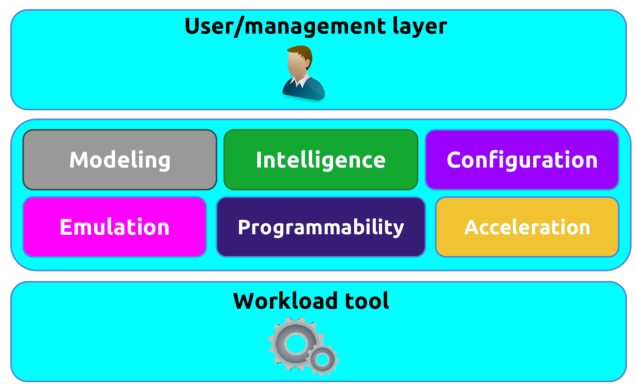
\includegraphics[height=2.4in]{figures/ch1/layer-diagram}
        \caption{ Architecture conceptual idea: a toll to automatize many tasks on traffic modelling and generation.}
    \label{fig:layer-diagram}
\end{figure*}



Now, we are going to formalize these exposed conceptual gaps in the literature, in a proposal of research and development. Or main targets here are:

\begin{itemize}


\item Survey the available open-source Ethernet workload tools available, addressing different features available;


\item Define what is a realistic Ethernet traffic, and the main approaches found in literature for crafting it;


\item Create a general method for modeling and parameterization of Ethernet traffic, aiming to mimic any traffic provided as input;


\item Create a software \textit{tool} able of \textit{learning} patterns and characteristics of real network traffic traces, and based on the acquired knowledge, allowing to reproduce network traffic with similar (but not equal) characteristics, \textit{avoiding} the storage of \textit{pcap} files. It must have a flow-oriented operation, and be able to choose the best features to represent each flow traffic. It will generate realistic Ethernet traffic based on these features learned, using available open source tools and APIs;


\end{itemize}


We call our  tool \textit{SIMITAR}, an acronym for \textit{SnIffing, ModellIng and TrAffic geneRation}.  These targets summarize a target of research, based on what we have exposed until now. We also will define some extra features, we want to have on our tool:

\begin{itemize}


\item Traffic Flow Programmability: the tool records this parameterization on a light-weight and human-readable version of a \textit{pcap} file. So the user can create his own models of traffic based on flows, in a platform-independent manner. He will not have to learn how to configure and script each tool.


\item Easy expansion: The sniffing, modeling, and traffic generation processes must work separately, so updates will be easy to manage. Also, the traffic generation is flow-oriented (it generates each flow individually). Thus the scheduling of each flow is platform-independent. In this way, is much easier to expand the support for new traffic generation engines.

\end{itemize}


Our goal is to offer an easier configuration, with a reasoble degree of realism than the available platforms today, at a reasonable speed. To do this, we are introducing the concept of programmability for  traffic generation. With SIMITAR, user may program its own synthetic traffic in a platform agnostic way. The intermediate layer of the figure ~\ref{fig:layer-diagram} summarize, the goal of the project in an illustrative way.


Instead of storing a file huge \textit{pcap} with a size of many \textit{gigas}, we create a light-weight set of models and parameters that describe this same trace. This tool will store the generalized set of parameters in a human and machine readable XML file we call \textit{Compact Trace Descriptor} (\textit{CTD}). Then, we use this data as input for a traffic generator engine. We do so using APIs or creating new processes in a controlled manner. So will be possible to control packet parameters and flow's behavior in a automatized and self-configuring way.


Using a component methodology, we decouple the traffic generation, from the data collection and parameterization process. Building it in this non-monolithic way,  enable a simple port for different traffic generators engines, what make our tools easy for updating with newer technologies. A project guideline is to reuse as much code and components as possible from the open-source community.


Now, we are going to formalize these exposed concepts in a proposal of research and development. Or main targets here are:

\begin{itemize}


\item Survey the available open-source Ethernet workload tools available, addressing its different features;


\item Define what is a realistic Ethernet traffic, and the man approaches found in literature;


\item Create a general method for modeling and parameterization of Ethernet traffic, aiming to mimic a provided input;


\item Create a software \textit{tool} able of \textit{learning} patterns and characteristics of real network traffic traces, and auto-configure the network traffic workloads, allowing to reproduce network traffic with similar (but not equal) characteristics, avoiding storage of \textit{pcap} files. 


\item It must have a flow-oriented operation, and be able to choose the best features to represent each flow traffic. It will generate realistic Ethernet traffic based on these features learned, using available open source tools and APIs;


\end{itemize}


%We also aim some advantages from the addition features: data visualization, packet acceleration, and distributed operation. Providing data visualization, it will not just work as a workload generator, but as a benchmark tool, providing statistics and performance analysis. Using packet acceleration, we will be able to produce a high throughput at the wire, and at the same time generate a trace as realistic as possible. Through a distributed operation of multiple instances, it will be easier to control its operation in a virtualized environment.  Finally, a project guideline is to reuse as much code and components as possible from the open-source community.


%3nd-review
\section{Document Overview}


In this introductory chapter, we presented an abstract of the state of the art, a problem statement, and proposed an approach for research and requirements for development.

%2nd-review
In the chapter section~\ref{ch:literature-review}, we go deeper on some subjects mentioned here. First, we present an extensive survey on open-source traffic generator tools. We summarize the benefits, and features supported by each one. After, we present a brief survey of important topics on realistic traffic generation. We are defining some important concepts we are going to use in this work, such as self-similarity, and heavy-tailed functions. Then, we discuss some techniques of validation of traffic generator tools and some practical examples. We also will make an analizis of some related works. 

%2nd-review
Chapter ~\ref{ch:architecture} introduces the methodology used in our project. We describe \textit{SIMITAR} low-level requirements and define an architecture and algorithms.  We also present its classes design and explain how \textit{SIMITAR} we can expand to any traffic generator engine with an API, CLI interface. We use the D-ITG API as an example. We explain its operation and suggest some use cases.

%2nd-review
In the chapter~\ref{ch:modeling-evaluation} we go deep in some subjects pointed in the previous chapter. We present how the modeling process actually works, using a defined data set (which we are going to use in the rest of the work). We also present some evaluation methods to check the modeling quality. We also describe our used and developed algorithms.

%2nd-review
In the chapter ~\ref{ch:validation}, we define a set of metrics based on previous tests on validation of traffic generators found in the literature. Here, we focus on packet, flow, and scaling metrics. we test \textit{SIMITAR} in an emulated SDN testbed with Mininet, using OpenDayLight as controller\cite{web-opendaylight}. 
 
%On chapter Use Cases~\ref{ch:use-cases}, we present two use cases of our tool. One using an NFV testbed, and other using an SDN p4 switch. Here we focus on QoS metrics, such as mean RTT. %use tools such as tcptrace and NFPA  on the use cases

%2nd-review
Finally, on chapter Conclusion and Future Work~\ref{ch:conclusion}, we summarized our work and highlights future works to improve \textit{SIMITAR} on realism and performance.

